



Flow in the sanitary sewer network can be classified as Dry-Weather Flow (DWF) and Wet-Weather Flow (WWF). DWF can be further divided in two components: 1. Base Waste Flow (BWF): inflow of waste water coming from households, commercial and industrial sites; and 2. Groundwater Infiltration (GWI): Water from aquifers that infiltrates into the network thought defects such as pipe cracks and leaky joints(Vallabhaneni and Burgess 2007). 
The choice of the hydrological model in this study aims the representation of RDII, which is the incremental flow into the sanitary sewer system caused by precipitation (rainfall or snowmelt). Figure 3 shows the typical characteristics of different components of sanitary sewer flow. RDII needs to be first separated from DWF when processing raw data coming from flow meters. More about the methods to separate the components are discussed on section 4.2.


\begin{figure}[ht]
    \centering
	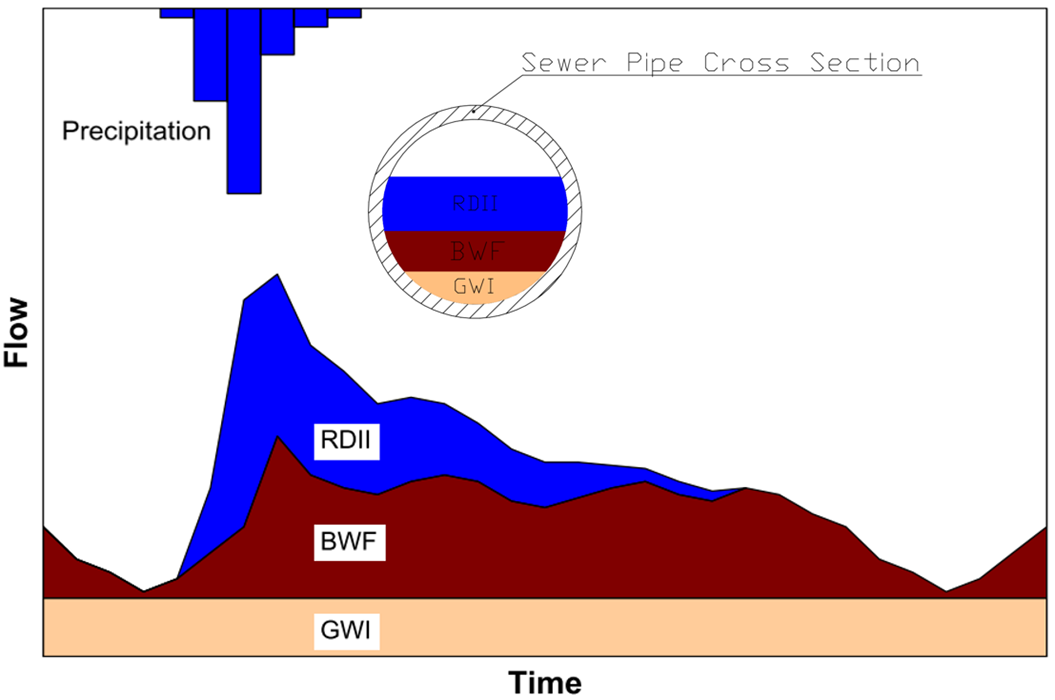
\includegraphics[scale=0.6]{figures/RDII_flows.png}
	\caption{Wet-weather flow components. Modified from \cite{Vallabhaneni2007}}
	\label{fig:flowcomponents}
\end{figure}


\begin{figure}[ht]
    \centering
	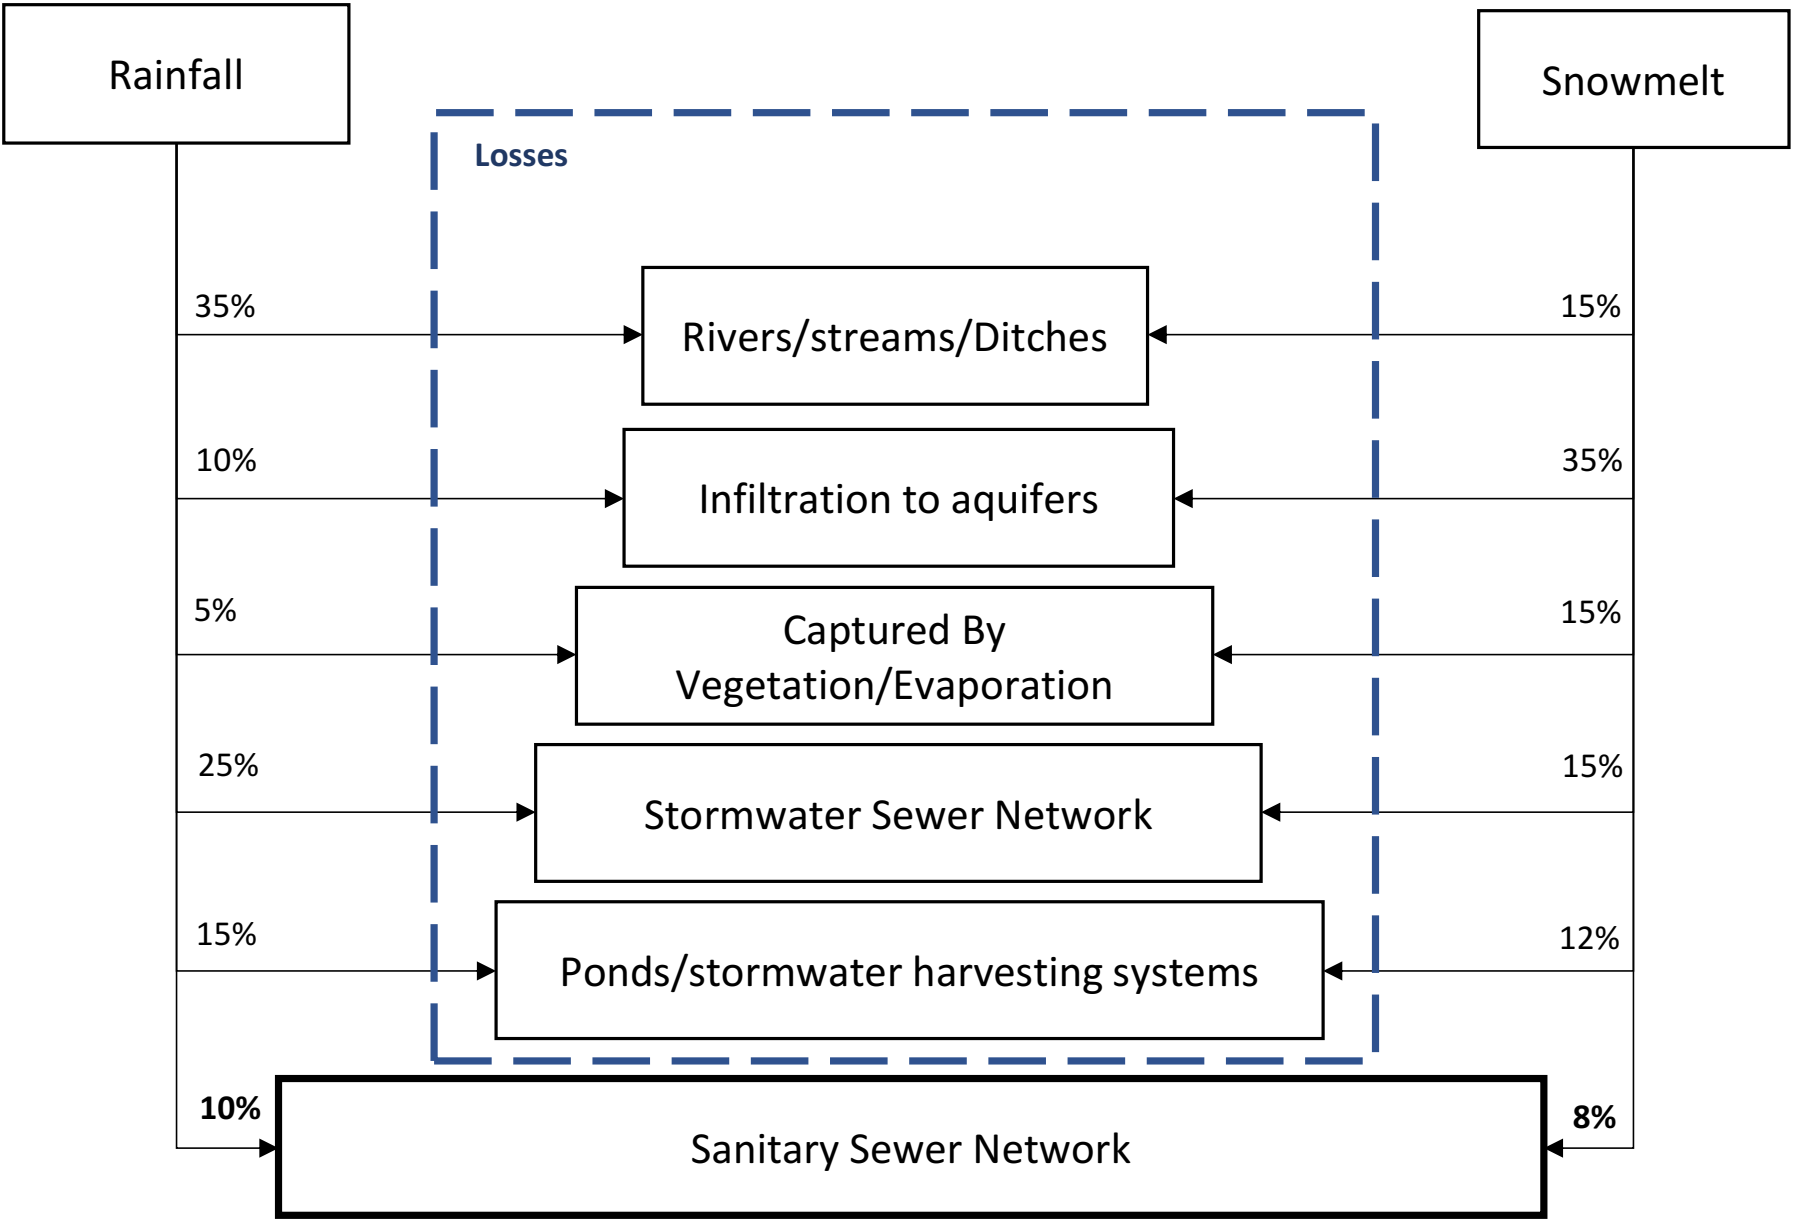
\includegraphics[scale=0.4]{figures/losses.png}
	\caption{Precipitation Losses relative to a Sanitary Sewer Network}
	\label{fig:losses}
\end{figure}

\section{Methods to Quantify Rainfall Dependent Infiltration and Inflow}


As mentioned on section 1. There are different ways stormwater or snowmelt finds its way into the sanitary sewer lines which ideally would have only wastewater from urban developments such as households, commercial centers, factories, etc.  Sanitary sewer networks’ flow increase can be trigged by an event such as a storm or elevation of the groundwater table. From rainfall or snowmelt water flows over the soil surface and inflows to the sanitary sewer through manhole leaky covers or directly from roof-drain and foundation connections. The flow increases in the sanitary sewer due to inflow is generally observed few hours after the beginning of the storm or snowmelt. As depicted in figure X, rainfall or snowmelt   Once the water infiltrates, it moves through the soil porous with a much slower velocity due to the characteristics of the groundwater flow. Infiltration of groundwater flow which reaches the elevation of pipe. Direct roof drain connections. Groundwater infiltration from saturated soil.   
There are many processes where. Function of the infiltration, groundwater flow, surface runoff, flow through pipe fissures.

Rainfall dependent infiltration and inflow have been modeled with different methods. Bennet (1999) (Bennett et al. 1999) carried a literature review and case study of around 10 different methods for quantifying RDII. 
The study concluded that only the regression and unit hydrograph methods are suitable when applying continuous simulation for long-term modelling. The unit hydrograph (UH) method also provided the best consistent match to storm peaks. Vallabhaneni and Burguess (2007) (Vallabhaneni and Burgess 2007) and U.S. EPA (2008) (Epa et al. n.d.) also considered sewer network rehabilitation capabilities as a factor for evaluation of the methods and suggested that regression should be used when more than 2 years of recorded flow and rainfall data is available. When no flow is available, the Constant Unit Rate RDII Method seems to be useful since it accounts for spatial characteristics of the Sewershed and information of pipe characteristics and population. Moreover, U.S. EPA (2008) study concluded that Unit Hydrograph RTK method can be useful to identify if which portion of the wet-weather flow is caused by inflow and which portion is caused by infiltration. Knowing whether RDII is more impacted by inflow or infiltration is relevant when evaluating the sanitary sewer network for rehabilitation. 
It is important to mention that the studies also concluded that there is no RDII quantification method that can be universally applied, since their use depend on available data and characteristics of the catchment. The goal of Vallabhaneni and Burguess (2007) (Vallabhaneni and Burgess 2007) and U.S. EPA (2008) (Epa et al. n.d.) reviews were to choose the most suitable method to be first implemented in a toolbox named as Sanitary Sewer Overflow Analysis and Planning (SSOAP). 




TELL HERE WHY THE CHOICE OF RDII AND SWMM

As described in section X. Two main reasons was to model snowmelt was the primary motivation to use SWMM modules and subcatchments in this study. and a model that could simulate the watershed behaviour throuout all the seasons of the year. 

\section{Physically-Based: SWMM Modules}

The use of SWMM packages in this study aimed to model four processes happening simultaneously in the watershed to simulate fast, medium and long term response observed in \ac{SSN} wet-weather flows. The four processes/SWMM modules are described here as: 1. Runoff; 2. Snowpack \& Snowmelt; 3. Infiltration; 4. Groundwater. 

\subsection{Rainfall-Runoff} 

\subsection{Snowpack \& Snowmelt} 

\subsection{Infiltration} \label{infiltration}

SWMM version 5.1 package offers the modeller five different infiltration models. The Modified Horton method \cite{akan1992,akan2003} was chosen among the options for three main reasons: 1. it is simply one of the default methods available in SWMM;  2. it has the same parameters as the well-known Horton method which parameter estimates are suggested in \citet{Rossman2016}; 3. Appears to be more accurate low intensity rainfall events than the original Horton method \cite{Rossman2016}. 

The two governing equations of the method describes the infiltration capacity decay during wet periods \ref{eqn:mhortondecay} and its recovery curve during dry periods \ref{eqn:mhortonrecoveryintegrated} and an example of these two curves and how the infiltration capacity would change over time is plotted in figure \ref{fig:horton}. 

\begin{figure}[h]
    \centering
	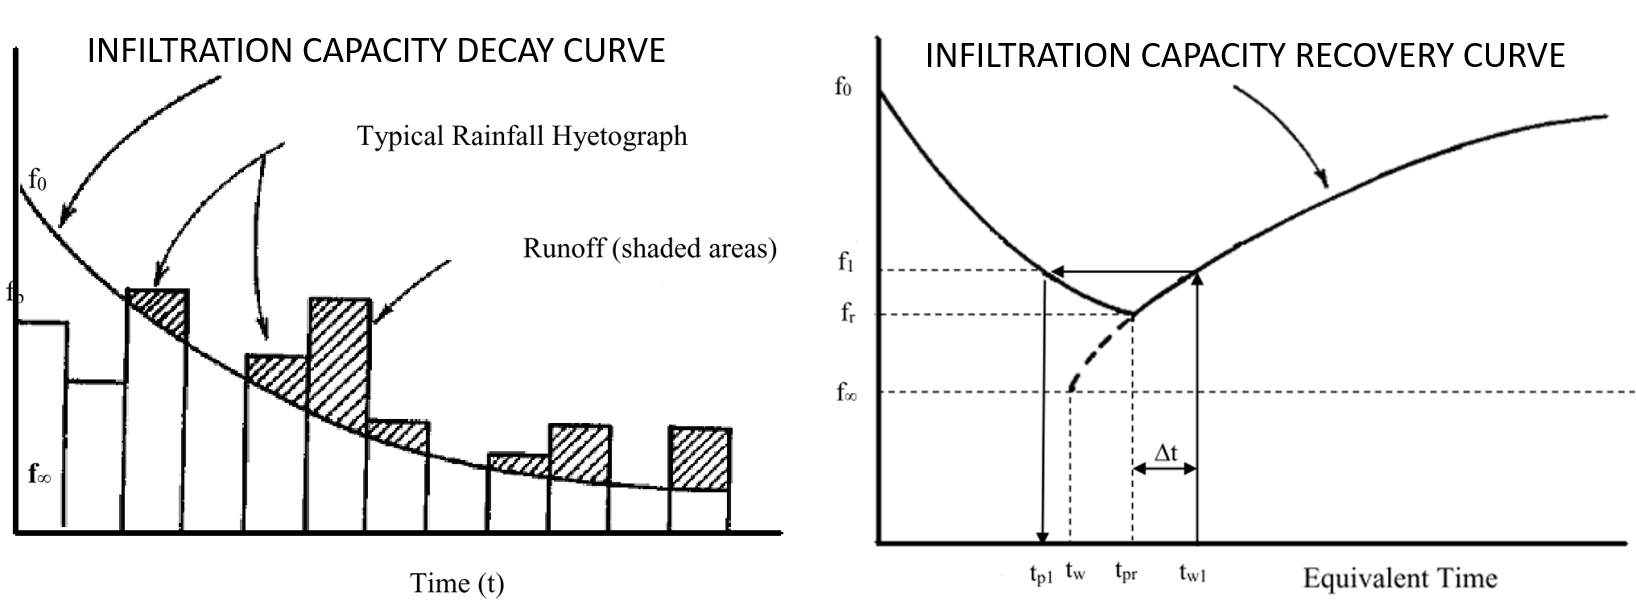
\includegraphics[scale=0.45]{figures/hortoncurves.png}
	\caption{Horton infiltration capacity decay and recovery curves. Modified from \cite{Rossman2016}}
	\label{fig:horton}
\end{figure}

\begin{equation}
\label{eqn:mhortondecay}
F = f_\infty \cdot t + \frac{(f_0 - f_\infty)}{k_d} \cdot (1 - e^{-k_d\cdot t})
\end{equation}
Where: \\
\indent $F$ = cumulative infiltration capacity [ft] \\
\indent $f_\infty$ = minimum or equilibrium value of infiltration capacity at $t = \infty$  [ft/sec] \\
\indent $f_0$ = maximum or initial value of infiltration capacity at $t = 0$ [ft/sec] \\
\indent $t$ = equivalent time [sec] \\
\indent $k_d$ = decay coefficient [sec\textsuperscript{-1}] \\

It is worth to mention that \ref{eqn:mhortondecay} is an integrated form of Horton's original equation. SWMM uses integrated form to consider the intensity of the rainfall event also as a function of the infiltration capacity reduction \cite{Rossman2016}. 


\begin{equation}
\label{eqn:mhortonrecovery}
\frac{df_r}{dt} = kr \cdot (f_0 - f_r) 
\end{equation}
Where: \\

\indent $f_r$ = infiltration capacity during recovery [ft] \\
\indent $f_{r0}$ = maximum or initial value of infiltration capacity at $t = 0$ [ft/sec] \\
\indent $k_r$ = regeneration coefficient [1/sec] \\
\indent $t$ = time [sec] \\

the infiltration capacity at time $t$ after integrating \ref{eqn:mhortonrecovery} when infiltration capacity is $f_{r0}$ is:

\begin{equation}
\label{eqn:mhortonrecoveryintegrated}
f_r =  f_0 - (f_0 - f_{r0}) \cdot e^{-k_d \cdot t}
\end{equation}
    
SWMM computation scheme first checks for wet-period (rainfall/snowmelt) or dry period to apply either of the equations \ref{eqn:mhortondecay} or \ref{eqn:mhortonrecoveryintegrated}  and compute the current infiltration capacity and the amount of water infiltrating the soil. More details of the equations and computational scheme are available in \citet{Rossman2016}.

Table \ref{tbl:infparam} presents a rough estimate of the range of four input parameters for Horton infiltration model. The range was extracted from EPA SWMM user help. 
 

\begin{table}[h]
\caption{Modified Horton infiltration parameters range\cite{Rossman2016}}
\label{tbl:infparam}
\centering
\begin{tabular}{@{}lcll@{}}
\toprule
\textbf{Parameter}        & \multicolumn{2}{c}{\textbf{Typical Range}} & \textbf{Units}        \\ \midrule
Maximum infiltration rate & \multicolumn{2}{c}{8.5 - 254}              & mm/h                  \\
Minimum infiltration rate & \multicolumn{2}{c}{0.254 - 120.4}          & mm/h                  \\
Decay coefficient         & \multicolumn{2}{c}{2 - 7}                  & h\textsuperscript{-1}\\
Drying Time               & \multicolumn{2}{c}{2 - 14}                 & days                  \\ \bottomrule
\end{tabular}
\end{table}




\subsection{Aquifer \& Groundwater Flow} 
 
choice of groundwater flow equation:


\section{Synthetic Unit Hydrograph: RTK}




\section{Separation of Flow Components}

•	SSOAP toolbox allows the users to visually adjust RTK parameters comparing the flow measured values and the RTK hydrograph through an iterative process \cite{Vallabhaneni2007}. Using such tool make the process easier for modelers. However, even with such tools, manual calibration can be time consuming. This can limit the frequency that calibrations are done. Optimization algorithm is applied as an attempt to mimic this iterative process done manually by modelers.

SSOAP Toolbox developed by \ac{EPA} has tools to support the quantification and management of RDII in sanitary sewer networks. The RDII Analysis Tool available in the SSOAP Toolbox can identify and separate DWF and WWF, determine parameters for the set of Unit Hydrographs RTK, and perform statistical analysis of the parameters to non-measured catchments and design storms (Vallabhaneni and Burgess 2007). The SSOAP was used in this study to quantify RDII, other two relevant features for the choice were: 1. free and open source; 2. Interface with SWMM 5.


\begin{figure}[ht]
    \centering
	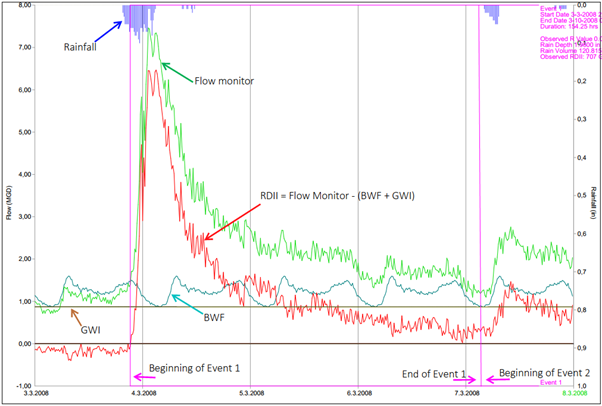
\includegraphics[scale=1.2]{figures/SSOAP_example.png}
	\caption{Graphical visualization of sanitary sewer flow components using SSOAP Toolbox}
	\label{fig:SSOAPexample}
\end{figure}
